\chapter{Confidence ($\mathcal{C}$)}
\label{ch:confidence}
%\begin{flushright}
%[TO-DO: quote]
%\end{flushright}
\minitoc

Pei Wang's uncertain logic is particularly elegant.  I adopt two ideas from his theory, explained below, but the way I use those numbers differs slightly from Wang's (cf his book \citep*{Wang2006} which describes an AGI called NARS (Non-axiomatic Reasoning System)).

\section{Positive and negative evidence}

In Wang's logic, each statement is attached with 2 numbers:\\
\hspace*{1cm} $w^+$ = number of positive examples\\
\hspace*{1cm} $w^-$ = number of negative examples\\
In an AGI system, they are the number of times a statement is observed to be true or false, respectively.

For example, for the statement\\
\hspace*{1cm} ``if X is female X probably has long hair''\\
the AGI may have observed 70 females with long hair and 30 females with short hair. The total \textbf{support} for the statement would be $(w^+ + w^-) = 100$ examples.

Using a pair of numbers allows us to know the probability of a statement as well as the the number of examples that support that statement. This is very important because some statements may be supported by very few examples and thus are ``weaker'' than statements with more support.

A major advantage of this 2-number approach is that probabilities can be updated by new examples. For example, if the AGI encounters a new female with long hair, it can update the probability easily with $ (w^+ + 1, \;w^-)$. Such updating cannot be done with the single-number representation of probability.

\section{Confidence}

Confidence is a concept borrowed from NARS.  In my terminology, the \textbf{support} of a statement is defined as:
\begin{equation}
w = w^+ + w^-
\end{equation}
which is an integer from 0 to $\infty$.

As Pei Wang did in NARS, the confidence $c$ is the value obtained by squashing $w$ into $[0,1]$, using a nonlinear transform such as:
\begin{equation}
 c = \frac{1}{1 + k/w} \hspace*{1.8cm}  \mbox{(Wang's method)}
\end{equation}
or \vspace{-0.3cm}
\begin{equation}
 c = 1 - e^{-ln2 \; \cdot \; (w / k)^2} \hspace*{1.2cm}  \mbox{(my method)}
\end{equation}
\vspace{-0.8cm}

\begin{figure}[H]
\centering
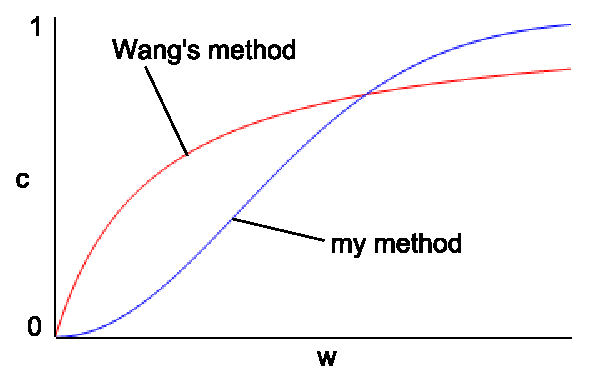
\includegraphics[scale=0.8]{Wang-vs-YKY-confidence-squashing-fn.eps}
% \caption{an example $\mathcal{P}(\mathcal{Z})$ distribution}
\end{figure}

An advantage of Wang's method is that it allows statements to have substantial confidence \textit{earlier} (so it gives nascent hypotheses more chance to succeed).  The advantage of my method is that it allows confidence to get closer to 1 sooner (so the incumbents have more strength).  The choice between these 2 may have interesting consequences in machine learning (see \S\ref{sec:confidenceInference}).

\section{Confidence and probability}

The probability (or frequency) of a statement is simply:
\begin{equation}
p = f = \frac{w^+}{w}
\end{equation}
Thus, $(w^+,w^-)$ contains information equivalent to the frequency and confidence pair $(f,c)$.

Notice that the confidence $c$ is \textit{orthogonal} to $f$ or $p$.  In \S\ref{sec:P(Z)-defined} we will see that each truth value in our logic is represented as a tuple: $(\mu, v, c)$ where $(\mu, v)$ describes a probability distribution and $c$ is the confidence.

\section{Confidence and logic}

To see how confidence is defined on logical formulae, it is easier to think in terms of the support $w$.  The support of a \textbf{rule} (ie, a logical formula containing variables) can be defined in a frequentist manner;  whereas the support of a \textbf{ground fact} (ie, a formula without variables) is always \textit{derived} from inference.

For example, the rule:\\
\hspace*{1cm} \textit{``Women usually have long hair''}\\
\hspace*{1cm} female(X) $\rightarrow$ long-hair(X)\\
is supported by a number of instances such as:\\
\hspace*{1cm} positive example: \hspace*{1cm} female(mary), long-hair(mary)\\
\hspace*{1cm} negative example: \hspace*{1cm} female(jane), $\neg$ long-hair(jane)\\
The support of the rule is the \textit{total} number of such instances that have been encountered\footnote{Here the Raven's paradox (or Hempel's paradox) is relevant:  Given the rule that ``women usually have long hair'' we can also state conversely that ``people with short hair are usually not women''.  Thus, a man with short hair would become a supportive example of this rule, which is counter-intuitive.  \{ TO-DO:  resolve this \}}.

A ground fact cannot be given the same treatment because it has no instances (being itself an instance) and its confidence must be inferred.  Inference of confidence is treated in \S\ref{sec:confidenceInference}.
